\documentclass{homework}

\title{Lab 10: BJT Amplifier Circuits}
\author{Kevin Evans}
\studentid{11571810}
\date{April 21, 2020}
\setclass{EE}{352}
\usepackage{amssymb}
\usepackage{mathtools}

\usepackage{amsthm}
\usepackage{amsmath}
\usepackage{slashed}
\usepackage{relsize}
\usepackage{threeparttable}
\usepackage{float}
\usepackage{booktabs}
\usepackage{boldline}
\usepackage{changepage}
\usepackage{physics}
\usepackage[inter-unit-product =\cdot]{siunitx}
\usepackage{setspace}

\usepackage[makeroom]{cancel}
\usepackage{pgfplots}

\usepackage{multicol}
\usepackage{tcolorbox}
\usepackage{enumitem}
\usepackage{times}
\usepackage{mhchem}
\usepackage{graphicx} 
\DeclareSIUnit{\year}{yr}
\usepackage{caption,subcaption} %multiline captions; subfigures
\begin{document}
	\maketitle
%	\vspace{-1em}
	\subsection*{Experiment 1: Single stage common emitter amplifier}
	In this experiment, a single stage CE amplifier was built in LTSPICE using the 2N3904 npn transistor. The amplifier was required to follow these specifications, \begin{itemize}
		\item Load resistance: \SI{47}{\kohm}
		\item Input resistance: exceeding \SI{1.2}{\kohm}
		\item Mid-band voltage gain: \SI{-85}{\V/\V} $\pm 20\%$
		\item Power supply voltage: \SI{12}{\V}
		\item Capacitances: $C_B = C_C = \SI{10}{\micro\farad}$, $C_E = \SI{47}{\micro\farad}$
	\end{itemize}

	\subsubsection*{DC biasing}
	This was done by first determining the bias points at DC and analyzing the circuit. Following the suggested base voltage $V_B = V_{CC} / 3$, a resistor divider was used to bias the base at \SI{4}{\V} using $R_1 = \SI{200}{\kohm}$ and $R_2 = \SI{100}{\kohm}$. %After finding the Thevenin equivalent of the base, 
	We can now solve for the emitter current by finding the Thevenin equivalent at the base. The base equivalent gives $V_{BB} = \SI{4}{\V}$ with a resistance of $R_{BB} = R_1 \parallel R_2$. For the current through the base-emitter junction, if we assume a constant drop of \SI{0.7}{\V}, then the DC emitter current can be found as  \begin{align*}
		0 & = V_{BB} - I_E R_{BB} - 0.7 - I_B R_E \\
			& = V_{BB} - I_E R_{BB} - 0.7 - \left(\beta + 1\right) I_E R_E \\
		I_E & = \frac{V_{BB} - 0.7}{R_{BB} / (\beta + 1) + R_E}
	\end{align*}
	If we choose $R_E$ as \SI{10}{\kohm}, the emitter current is approximately \SI{0.3093}{\mA} and an emitter voltage of \SI{3.093}{\V}, and a base voltage of \SI{3.793}{\V}. At this biasing point, the collector and base current can be found
	\begin{align*}
	I_C = \alpha I_E = \frac{\beta}{\beta + 1} I_E = \SI{0.3063}{\mA} && I_B = \frac{1}{\beta + 1}I_E = \SI{3.063}{\micro\ampere}
	\end{align*}
	From this, the BJT transconductance and incremental resistance is found at this current as \begin{align*}
		g_m & = \frac{I_C}{V_T} = \SI{12.25}{\mA/\V} \\
		r_o & = \frac{V_A}{I_C} = \SI{326}{\kohm} \\
		r_\pi & = \frac{V_T}{I_B} = \SI{8.162}{\kohm}
	\end{align*}

	\subsection*{AC analysis}
	The AC equivalent circuit can be found by shorting the capacitors and using the BJT small-signal equivalent. This is shown in Figure \ref{fig:screenshot001}.
	\begin{figure}[H]
		\centering
		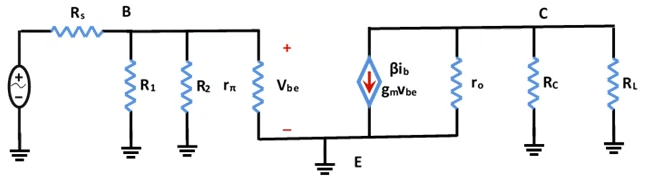
\includegraphics[width=0.7\linewidth]{screenshot001}
		\caption{AC equivalent circuit of the CE amplifier.}
		\label{fig:screenshot001}
	\end{figure}
	\noindent From the equivalent circuit, the input resistance is determined as 
	\[ R_I = r_\pi \parallel R_1 \parallel R_2 = \SI{7.3}{\kohm}\]
	which exceeds the requirement. The midband gain is required to be \SI{-85}{\V/\V} and will allow the collector resistance to be determined using the equivalent circuit, \begin{align*}
		G_v & = -g_m R_o \frac{R_i}{R_s + R_i}\\
		-85 & =  -0.01225 \times R_o \times 0.993 \\
		R_o & = \left(r_o \parallel R_C \parallel R_L \right) = \SI{7}{\kohm} \\
		R_C & = \SI{8.44}{\kohm}
	\end{align*}

	\subsubsection*{DC simulation and verification}
	Using the values determined, the DC circuit was built in LTSPICE and a transient analysis was done to verify the voltage, as shown in Figure \ref{fig:screenshot002}. The transistor voltage and currents were measured as \begin{align*}
		V_C & = \SI{9.23234}{\V} && I_C = \SI{329.483}{\micro\ampere} \\
		V_B & = \SI{3.93041}{\V} && I_B = \SI{1.04379}{\micro\ampere} \\
		V_E & = \SI{3.30527}{\V} && I_E = \SI{330.527}{\micro\ampere}
	\end{align*}
	These values were very close to the expected values. The differences are likely due to the changes $\beta$, which is roughly $300$ in LTSPICE, rather than the $100$ used in the calculations. At this bias point, the transconductance was estimated roughly $3.4\%$ from the expected value at
		\[ g_m = \frac{\SI{329.5}{\uA}}{\SI{26}{\mV}} = \SI{12.67}{\mA/\V} \]
	
	\subsubsection*{Amplifier simulation}
	The full amplifier circuit was built in LTSPICE, shown in Figure \ref{fig:screenshot002}, and simulated using a transient analysis for a duration of \SI{1}{\ms}. For an input of \SI{20}{\mV} (pp) at \SI{20}{\kHz}, the gain was measured as \begin{align*}
		G_v & = \frac{-1.76474}{0.020} = \SI{-88.2}{\V/\V}
	\end{align*}
	This gain of \SI{-88.2}{\V/\V} is within the specifications, at $3.8\%$ from the expected \SI{-85}{\V/\V}. As this is within the requirements, no trimming on $R_E$ or $R_C$ is needed. As we increase the input signal voltage, it begins to clip. The lower bound of the clipping is near the collector voltage at \SI{3.4}{\V} and the upper bound is near \SI{11.6}{\V}. The maximum voltage swing is \SI{2.4}{\V} at the emitter, or \SI{66}{\mV} at the base. 
	
	The input resistance by measuring the voltage and current at the base, \begin{align*}
		R_i & = \abs{ \frac{V_b}{i_s} } = \frac{\SI{20}{\mV}}{\SI{1.21}{\micro\ampere}} = \SI{16.5}{\kohm}
	\end{align*}
	This input resistance exceeds the specification of \SI{1.2}{\kohm} and exceeded the predicted value.
	The frequency response was obtained from \SI{10}{\Hz} to \SI{10}{\MHz} and is shown in Figure. The cutoff frequencies were measured \begin{align*}
		f_L = \SI{43.0}{\Hz} && f_H = \SI{5.82}{\MHz}
	\end{align*}
	When the emitter resistor is split into \SI{47}{\ohm} and \SI{9953}{\ohm}, the new gain and input resistance was measured \begin{align*}
		G_v = \frac{-1.1187}{0.020} = \SI{56}{\V/\V} && R_i = \frac{\SI{20}{\mV}}{\SI{863.252}{\nA}} = \SI{23.2}{\kohm}
	\end{align*}
	This is a $37\%$ drop from the original gain, and an increase of input resistance. The change in the gain is due to the AC signal dropping across the new \SI{47}{\ohm} resistor, instead of bypassing the emitter resistors through the capacitor.
	
	
	\subsection*{Experiment 2: Basic Differential Amplifier}
	The differential amplifier circuit was created in LTSPICE. Initially, the DC circuit was simulated using a transient analysis to measure the output voltage as 
	\[ V_o = \SI{5.32}{\V} \]
	The differential gain for this amplifier should be roughly \begin{align*}
		A_d & = \frac{1}{2} g_m ( r_o \parallel R_2 ) = -\frac{1}{2} \frac{I_c}{V_T} (r_o \parallel R_2) \\
			& \approx \SI{88.9}{\V/\V}
	\end{align*}
	In LTSPICE, the differential gain was measured, with a test voltage $V_d = \SI{20}{\mV}$ (pp) applied across the $V_i^+$ and $V_i^-$ terminals and the gain was measured as
	\[ A_d = \frac{1.695}{0.020} \approx \SI{85}{\V/\V} \]
	Then, the common mode gain was measured using a test voltage $V_{cm} = \SI{1}{\V}$ (pp) applied to both input terminals. Using a transient simulation, the gain was measured,
	\[ A_{CM} = \frac{-0.495}{1.000} = -0.495\]
	This was fairly close to the expected common mode gain of $-0.5$. The common mode rejection ratio can now be found as
	\[\mathrm{CMRR} = 20 \log(A_d / A_{cm}) = \SI{44.7}{\dB} \]
	
	
	\subsection*{Experiment 3: Improved Differential Amplifier}
	If we assume the current mirror is ideal with matched transistors, then the current across each emitter (and the resistor) is \begin{align*}
		I_R & = \SI{0.93}{\mA} = \frac{10 - 0.7 - (-10)}{R} \\
		\implies R & = \SI{20.75}{\kohm}
	\end{align*}
	Then, we can determine the DC currents through the original two transistors and determine the new transconductance values, \begin{align*}
		I_1 = I_2 & = I_R / 2 \\
		I_1 = I_2 & = \SI{0.465}{\mA} \\
		g_m & = \SI{18.6}{\mA/\V}
	\end{align*}
	In LTSPICE, the circuit was simulated at DC with both inputs grounded. The output voltage was found using a transient analysis as 
	\[ V_o \approx \SI{5}{\V} \]
	Next, a \SI{20}{\mV} (pp) sine wave was applied across the differential input and the gain was calculated, quite close to the original amplifier, as
	\[ A_d = \frac{1.82}{0.02} \approx \SI{91}{\V/\V}  \]
	The common-mode gain was tested using the approach as earlier and the common mode gain was calculated as
	\[ A_{cm} = \frac{\num{915e-6}}{0.02} = \SI{0.046}{\V/\V} \]
	The CMRR was recalculated with these new values as \begin{align*}
		\mathrm{CMRR} & = 20 \log(A_d / A_{cm}) = \SI{66.0}{\dB} 
	\end{align*}
	The new CMRR is improved substantially compared to the original CMRR, nearly \SI{20}{\dB} higher. This improvement is due to the fact that there is more control over the current because of the added current mirror. A larger change in the input signal voltage no longer affects the bias current significantly, since the bias current is primarily controlled through the mirror. 
	\subsection*{Appendix}
	\begin{figure}[H]
		\centering
		\begin{subfigure}{0.4\linewidth}
			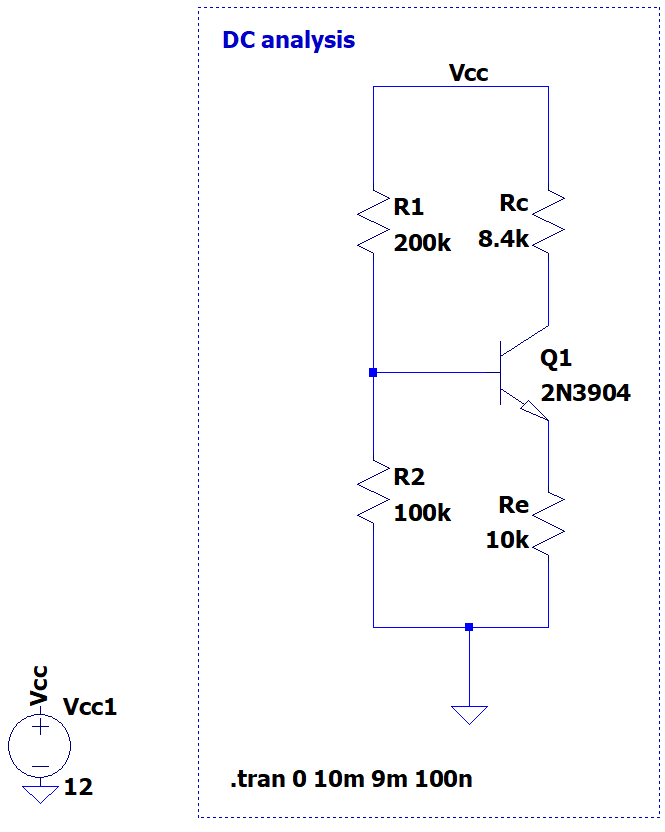
\includegraphics[width=\linewidth]{screenshot002}
		\end{subfigure}
		\hfil
		\begin{subfigure}{0.5\linewidth}
			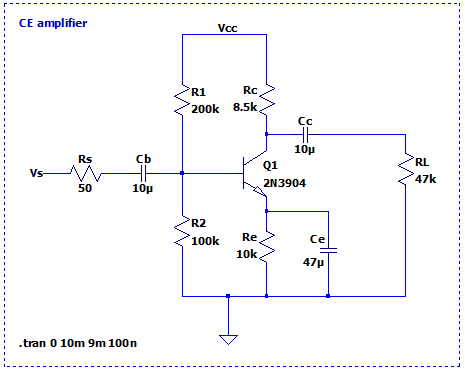
\includegraphics[width=\linewidth]{screenshot003}
		\end{subfigure}
		\caption{DC and AC circuits built and simulated in LTSPICE.}
		\label{fig:screenshot002}
	\end{figure}


\end{document}